\documentclass[11pt]{article}

\usepackage{times}
\usepackage{epsfig}
\usepackage{natbib}
\usepackage{amsmath, amssymb, amstext}
\usepackage{bm}
\usepackage{cancel}

\begin{document}

\begin{figure}[htbp]
  \centerline{ 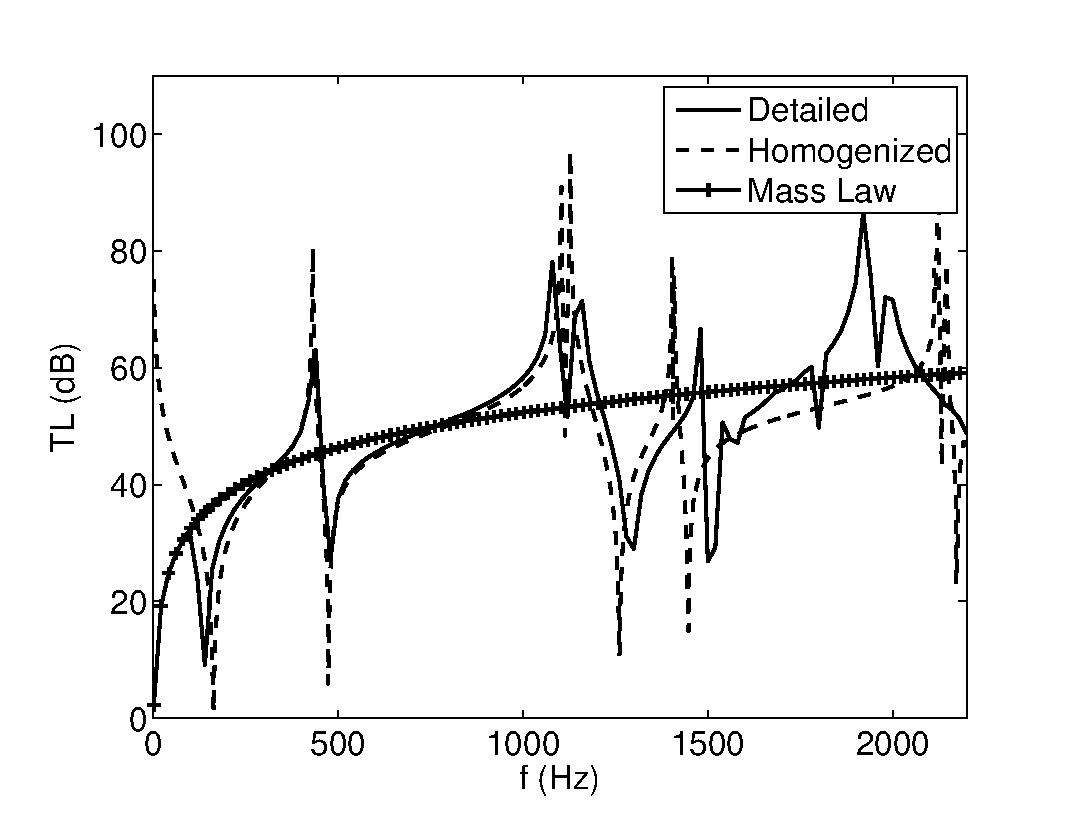
\epsfig{file=6mmResTc.eps, scale=0.5} }
  \caption{6mm Resonator Tc}
  \label{fig:6mmTc}
\end{figure}

\begin{figure}[htbp]
  \centerline{ 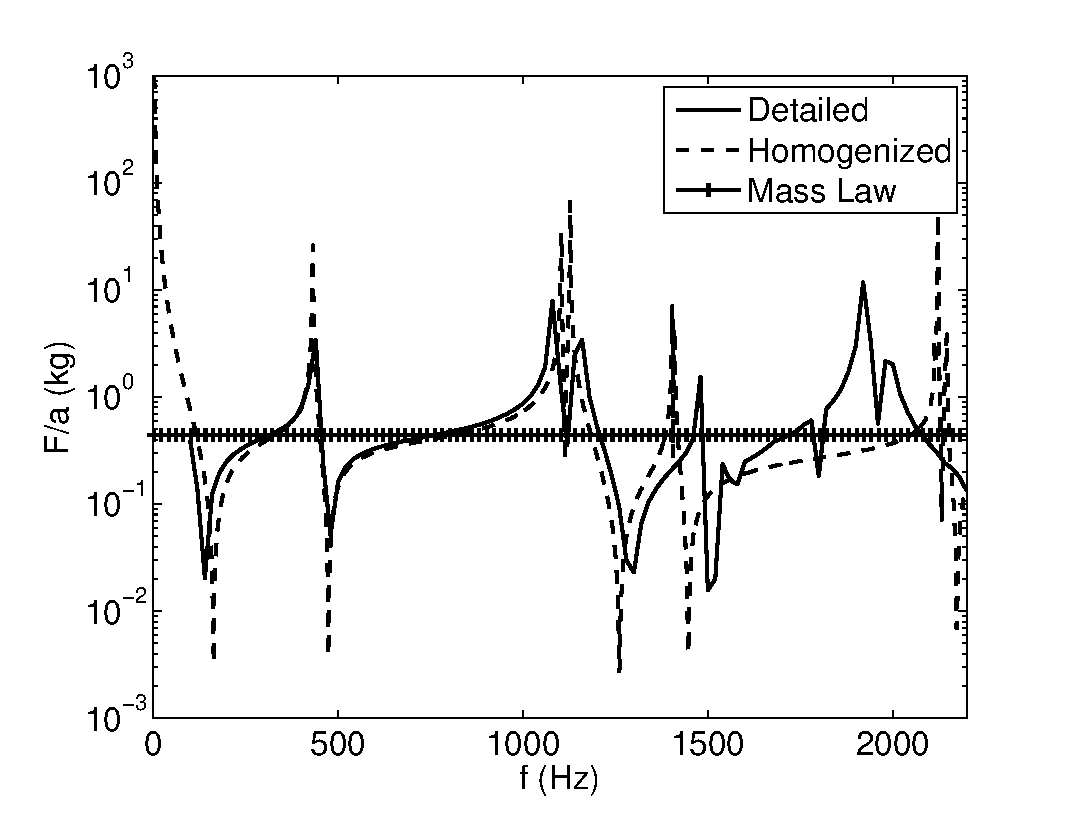
\epsfig{file=6mmResFa.eps, scale=0.5} }
  \caption{6mm Resonator Fa}
  \label{fig:6mmFa}
\end{figure}

\begin{figure}[htbp]
  \centerline{ 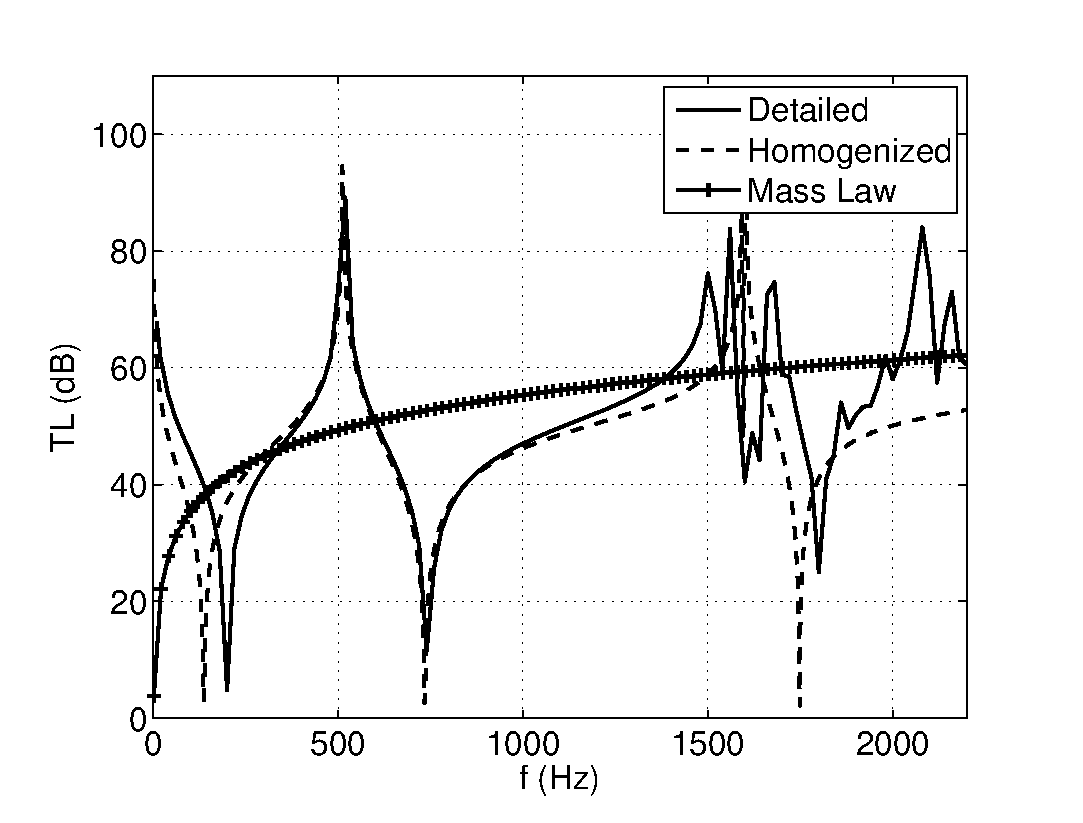
\epsfig{file=10mmResTc.eps, scale=0.5} }
  \caption{10mm Resonator Tc}
  \label{fig:10mmTc}
\end{figure}

\begin{figure}[htbp]
  \centerline{ 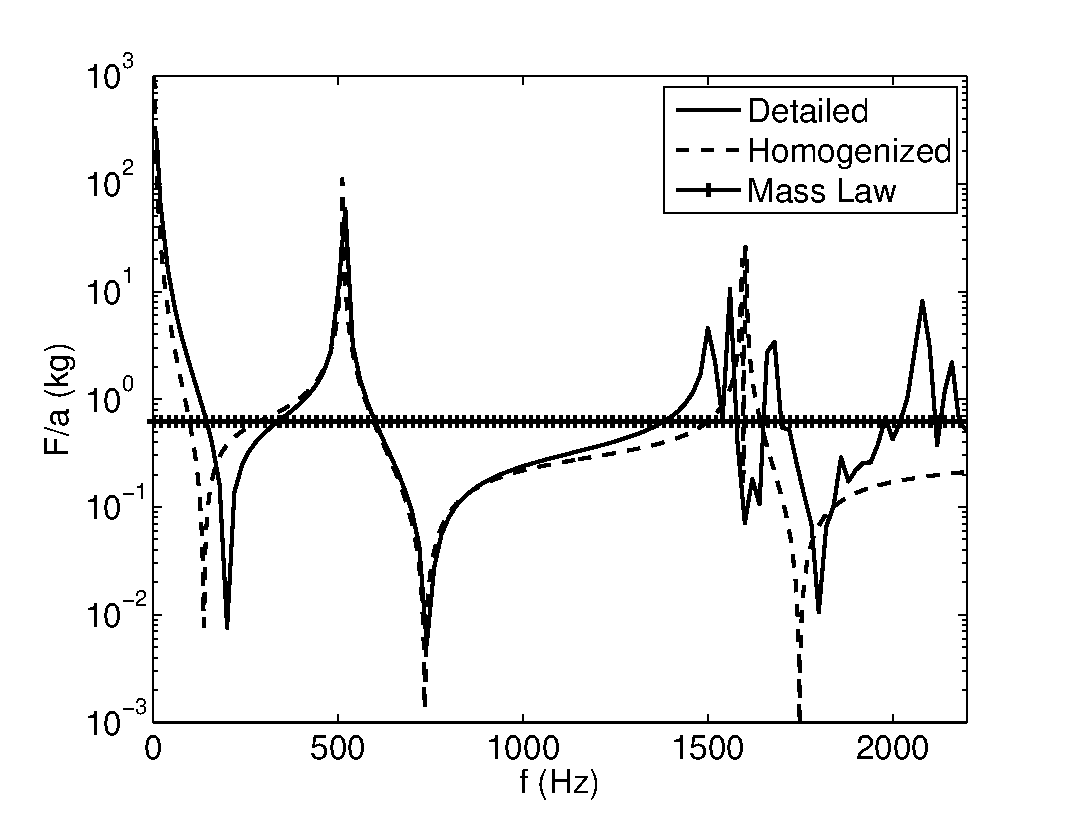
\epsfig{file=10mmResFa.eps, scale=0.5} }
  \caption{10mm Resonator Fa}
  \label{fig:10mmFa}
\end{figure}

\begin{figure}[htbp]
  \centerline{ 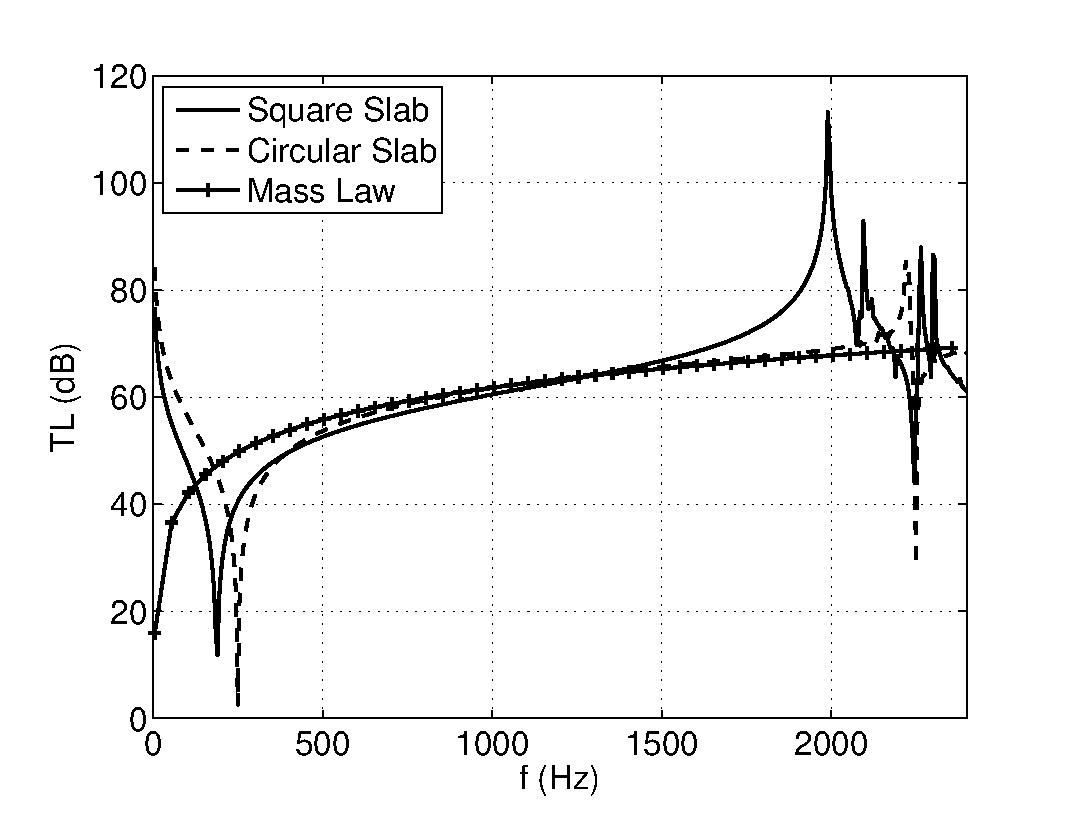
\epsfig{file=SlabSqrCirc.eps, scale=0.5} }
  \caption{Comparison of Circular and Square Slabs}
  \label{fig:SqrCirc}
\end{figure}

\begin{figure}[htbp]
  \centerline{ 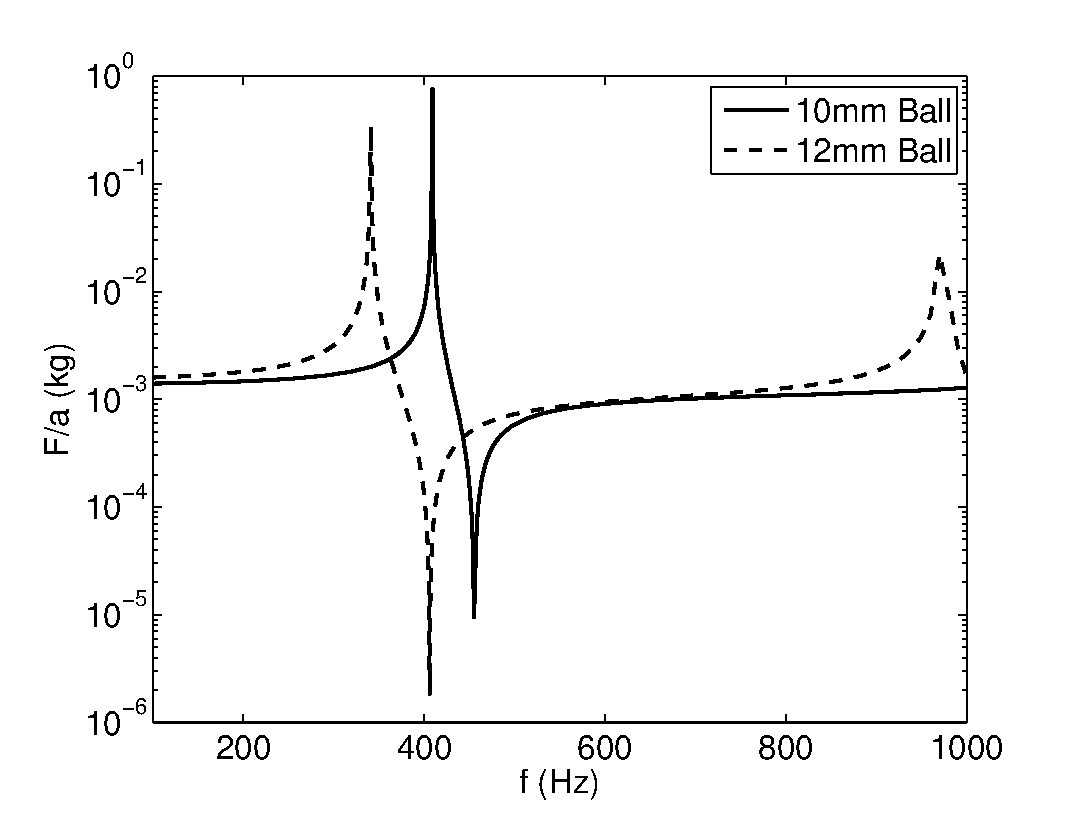
\epsfig{file=TwoRes.eps, scale=0.5} }
  \caption{Two Sizes of Steel Balls}
  \label{fig:TwoRes}
\end{figure}

\begin{figure}[htbp]
  \centerline{ 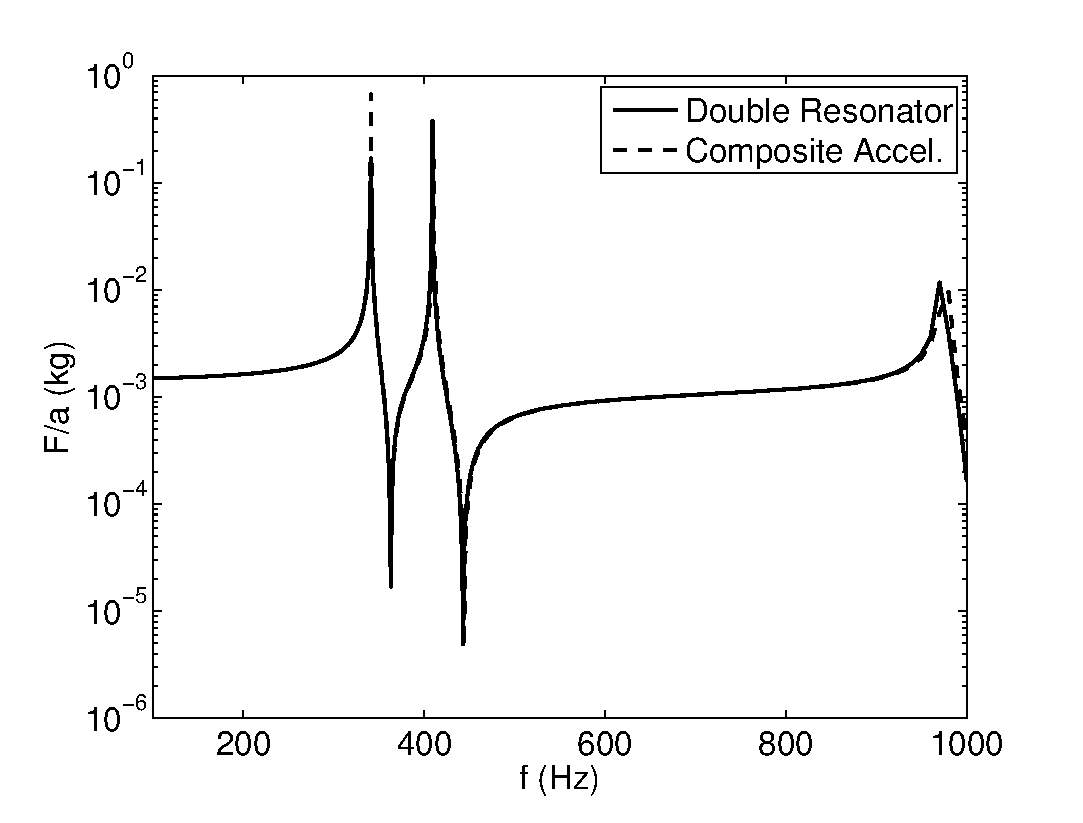
\epsfig{file=DoubleRes.eps, scale=0.5} }
  \caption{Composite vs. Double Resonator}
  \label{fig:DoubleRes}
\end{figure}

\end{document}



